% A2 portrait poster. Build: cd poster && latexmk -xelatex poster.tex
% Figures: .venv/bin/python poster/make_figures.py (from the repository root)
\documentclass{article}
\usepackage[paperwidth=420mm,paperheight=594mm,margin=14mm]{geometry}
\usepackage{fontspec}
\setmainfont{Inter}[Numbers=Lining]
\usepackage{xcolor}
\usepackage{graphicx}
\usepackage{tikz}
\usetikzlibrary{arrows.meta,positioning,calc}
\usepackage[most]{tcolorbox}
\usepackage{enumitem}
\usepackage{qrcode}
\usepackage{microtype}
\usepackage{amssymb}
\usepackage{ragged2e}

\definecolor{accent}{HTML}{2A78D6}
\definecolor{ink}{HTML}{0B0B0B}
\definecolor{ink2}{HTML}{52514E}
\definecolor{wash}{HTML}{EDF4FD}
\definecolor{line}{HTML}{D9D8D2}

\pagestyle{empty}
\hyphenpenalty=10000
\exhyphenpenalty=10000
\setlength{\parindent}{0pt}
\setlength{\parskip}{0pt}
\color{ink}

% Type sizes for A2 read from about 1 m.
\newcommand{\bodysize}{\fontsize{18}{23}\selectfont}
\newcommand{\smallsize}{\fontsize{14}{18}\selectfont}
\newcommand{\headsize}{\fontsize{28}{34}\selectfont}

\setlist[itemize]{leftmargin=1.1em,itemsep=5pt,topsep=3pt,parsep=0pt,
  label={\color{accent}\raisebox{0.12em}{\scalebox{0.8}{$\blacksquare$}}}}

% A titled poster section with a short accent rule above the title.
\newtcolorbox{pbox}[2][]{enhanced,colback=white,colframe=white,
  boxrule=0pt,left=0mm,right=0mm,top=1mm,bottom=1mm,arc=0mm,
  before skip=0mm,after skip=0mm,fontupper=\bodysize\RaggedRight,
  title={\headsize\bfseries #2},coltitle=accent,colbacktitle=white,
  toptitle=4mm,bottomtitle=2mm,
  overlay={\draw[accent,line width=1.2mm] (frame.north west) -- ++(25mm,0);},
  #1}

\newcommand{\finding}[1]{{\fontsize{20}{25}\selectfont\bfseries #1\par}\vspace{1mm}}
\newcommand{\note}[1]{\par\vspace{1mm}{\smallsize\color{ink2}#1\par}}

\newlength{\colw}
\setlength{\colw}{\dimexpr(\textwidth-14mm)/2\relax}
\newcommand{\rowgap}{\par\vspace{3mm}}

\begin{document}
\bodysize

% ------------------------------------------------------------------ header
\begin{tcolorbox}[enhanced,colback=accent,colframe=accent,arc=0mm,boxrule=0pt,
  left=10mm,right=10mm,top=5mm,bottom=4mm,width=\textwidth,before skip=0mm,after skip=0mm]
\color{white}
{\fontsize{48}{54}\selectfont\bfseries Released trees leak training records,\\
and the attacker knows which ones\par}
\vspace{2mm}
{\fontsize{22}{28}\selectfont Reconstructing training data from a published Rashomon set of decision trees\par}
\vspace{3mm}
{\fontsize{21}{26}\selectfont\bfseries Hendrik De Coster \quad Francesco Fuligni \quad Aurélien Craplet\par}
\vspace{1mm}
{\fontsize{18}{23}\selectfont Department of Computer and Systems Sciences (DSV), Stockholm University
\,·\, Research Topics in Data Science 2026\par}
\end{tcolorbox}
\rowgap

% ------------------------------------------------------- intro and question
\begin{minipage}[t]{\colw}\vspace{0pt}
\begin{pbox}{Why it matters}
\begin{itemize}
\item Interpretable decision trees get published for transparency; a
  \textbf{Rashomon set} holds all near-optimal trees [4].
\item Each tree reveals how many training rows fall in every leaf; together,
  the counts pin down the training table [1--3].
\item Earlier attacks report one error for the whole table, so the attacker
  cannot tell \emph{which} rebuilt rows are real people.
\end{itemize}
\end{pbox}
\end{minipage}\hfill
\begin{minipage}[t]{\colw}\vspace{0pt}
\vspace{3mm}
\begin{tcolorbox}[enhanced,colback=wash,colframe=wash,arc=2mm,boxrule=0pt,
  left=5mm,right=5mm,top=4mm,bottom=4mm,fontupper=\bodysize\RaggedRight,before skip=0mm,after skip=0mm]
{\headsize\bfseries\color{accent} Research question\par}\vspace{2mm}
{\fontsize{21}{27}\selectfont\bfseries When $m$ trees of a Rashomon set are
released, how many training records can an attacker rebuild, and can it
tell which ones are right?\par}
\vspace{2mm}
\begin{itemize}
\item[\textbf{1}] How do $m$ and background knowledge affect the error?
\item[\textbf{2}] Can each record get a confidence that is calibrated
  without ground truth?
\end{itemize}
\end{tcolorbox}
\end{minipage}
\rowgap

% ------------------------------------------------------------------ method
\begin{pbox}{Method}
\centering
\begin{tikzpicture}[
  box/.style={draw=line,line width=0.8mm,rounded corners=3mm,fill=white,
    align=center,text width=61mm,minimum height=27mm,inner sep=2mm,
    font=\fontsize{16}{20}\selectfont},
  key/.style={box,draw=accent,fill=wash},
  arr/.style={-{Latex[length=6mm,width=5mm]},line width=1mm,color=ink2},
  node distance=11mm]
\node[box] (data) {\textbf{Private data}\\100 rows of UCI Adult,\\13 binary columns + income};
\node[box,right=of data] (set) {\textbf{Rashomon set}\\all trees within 10\%\\of the best (TreeFARMS)};
\node[box,right=of set] (rel) {\textbf{Release}\\$m$ trees drawn at random,\\with their leaf counts};
\node[key,right=of rel] (out) {\textbf{Attack (CP-SAT)}\\20 tables that fit every\\leaf count, guided by\\2,000 public records};
\node[key,right=of out] (conf) {\textbf{Output}\\100-row table; a row's\\confidence = share of\\the 20 tables with it};
\draw[arr] (data) -- (set);
\draw[arr] (set) -- (rel);
\draw[arr] (rel) -- (out);
\draw[arr] (out) -- (conf);
\end{tikzpicture}
\par\vspace{4mm}\raggedright
{\fontsize{17}{22}\selectfont \textbf{Prior-guided sampling:} each table is the
consistent table closest to a random draw from the public records.
\textbf{Baseline:} public statistics only, no trees. \textbf{RQ1:} also knows
columns A, B; $m$ = 1--200, 100 seeds. \textbf{RQ2:} $m$ = 10--100, 20 seeds.\par}
\end{pbox}
\rowgap

% ----------------------------------------------------------------- results
\begin{minipage}[t]{\colw}\vspace{0pt}
\begin{pbox}[equal height group=r1]{Result 1 · The trees leak records}
\finding{With 50 trees the attacker vouches for 45\% of the rows, and 98\% of
those are right.}
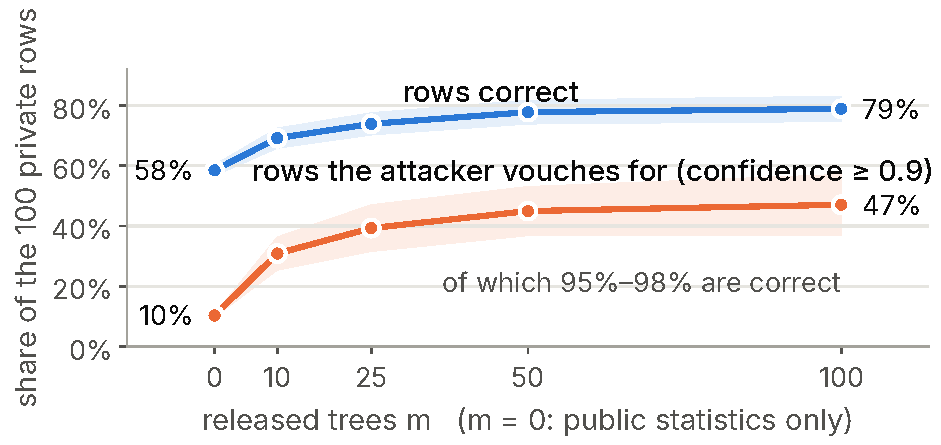
\includegraphics[width=\linewidth]{figures/leak_vs_m.pdf}
\note{20 seeds (18 at $m$ = 100), 95\% intervals; correct = every column matches.}
\end{pbox}
\end{minipage}\hfill
\begin{minipage}[t]{\colw}\vspace{0pt}
\begin{pbox}[equal height group=r1]{Result 2 · The attacker knows which}
\finding{Stated confidence matches accuracy with no fitting: off by only
0.7--2.3 points at every $m$.}
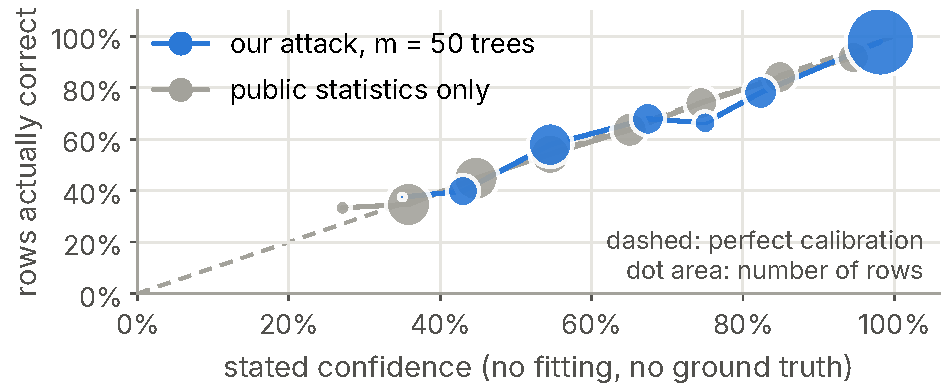
\includegraphics[width=\linewidth]{figures/reliability_m50.pdf}
\note{All 2,000 rows of 20 seeds at $m$ = 50, grouped by stated confidence.}
\end{pbox}
\end{minipage}
\rowgap

\begin{minipage}[t]{\colw}\vspace{0pt}
\begin{pbox}{Result 3 · Knowing more barely helps}
\finding{200 trees cut the error on sex from 0.35 to 0.25; two known
attributes save about 1 point more.}
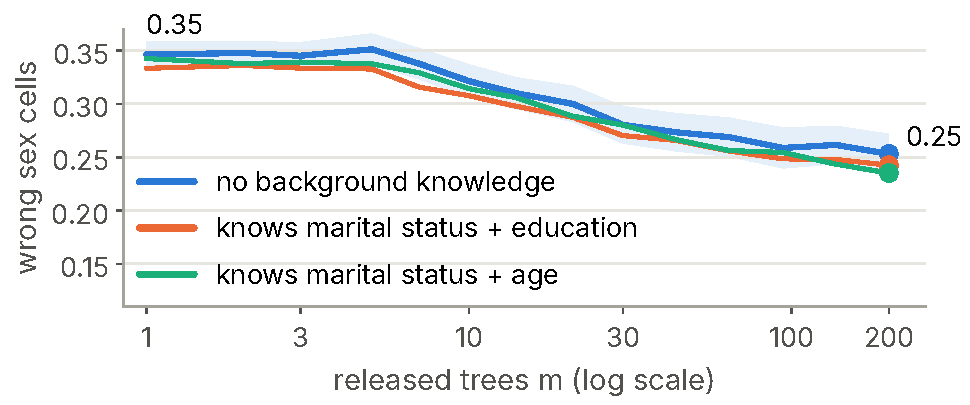
\includegraphics[width=\linewidth]{figures/background_knowledge.pdf}
\note{A = marital status, B = education or age; 100 seeds; band: 95\% interval.}
\end{pbox}
\end{minipage}\hfill
\begin{minipage}[t]{\colw}\vspace{0pt}
\begin{pbox}{Result 4 · What changes the answer}
\begin{itemize}
\item \textbf{Which trees:} TreeFARMS lists near-copies first; releasing the
  first $m$ trees understates the leak by 8--12 points.
\item \textbf{Scarce public data:} with 200 public records the attack is \mbox{6--9}
  points overconfident; a Dirichlet prior brings this to 2, at equal accuracy.
\end{itemize}
\end{pbox}
\vspace{5mm}
\begin{pbox}{Conclusion and future work}
\begin{itemize}
\item More released trees leak more records, and the attacker knows which.
\item Judge privacy risk per record, not by one table-wide error.
\item \textbf{Next:} differentially private leaf counts, larger tables,
  public data from another population.
\end{itemize}
\end{pbox}
\end{minipage}
\rowgap

% ---------------------------------------------------------------- footer
\begin{pbox}[toptitle=3mm,bottomtitle=1mm]{References and code}
\begin{minipage}[t]{\dimexpr\linewidth-88mm\relax}\vspace{0pt}
\fontsize{12.5}{15.5}\selectfont
\begin{enumerate}[leftmargin=2em,itemsep=2pt,topsep=0pt,label={[\arabic*]}]
\item J. Ferry, U. Aïvodji, S. Gambs, M.-J. Huguet, M. Siala. Probabilistic
  dataset reconstruction from interpretable models. \emph{IEEE SaTML}, 2024.
\item J. Ferry, R. Fukasawa, T. Pascal, T. Vidal. Trained random forests
  completely reveal your dataset. \emph{ICML}, 2024.
\item E. Hsu, H. Chen, C. Zhong, L. Semenova. The double-edged nature of the
  Rashomon set for trustworthy machine learning. \emph{ICML}, 2026.
\item R. Xin, C. Zhong, Z. Chen, T. Takagi, M. Seltzer, C. Rudin. Exploring
  the whole Rashomon set of sparse decision trees. \emph{NeurIPS}, 2022.
\item T. Dick, C. Dwork, M. Kearns, T. Liu, A. Roth, G. Vietri, Z.\,S. Wu.
  Confidence-ranked reconstruction of census microdata from published
  statistics. \emph{PNAS}, 2023.
\end{enumerate}
\end{minipage}\hfill
\begin{minipage}[t]{84mm}\vspace{0pt}
\begin{minipage}[t]{42mm}\vspace{0pt}{\fontsize{14}{18}\selectfont\bfseries
Code, data and results\par}\vspace{2mm}{\fontsize{12.5}{16}\selectfont
github.com/\\francescofuligni/\\rtds-project\par}\end{minipage}\hfill
\begin{minipage}[t]{36mm}\vspace{0pt}\qrcode[height=36mm]{https://github.com/francescofuligni/rtds-project}\end{minipage}
\end{minipage}
\end{pbox}

\end{document}
